\newcommand{\notacontroles}{\caption*{\footnotesize Fuente: Precios históricos de bencinaenlinea.cl. Log del precio $\times$ 100. Control $>$3 km: estaciones sin entradas a menos de 3 km (amplio), control $>$5 km: sin entradas a menos de 5 km (estricto). Errores estándar agrupados por comuna entre paréntesis. * p$<$0,10 ** p$<$0,05 *** p$<$0,01. Bins de seis meses desde la entrada, referencia en $-1$.}}
\newcommand{\notaes}{\caption*{\footnotesize Fuente: Precios históricos de bencinaenlinea.cl. Panel mensual 2012 a 2026, log del precio $\times$ 100. Errores estándar agrupados por comuna entre paréntesis. * p$<$0,10 ** p$<$0,05 *** p$<$0,01. Bins de seis meses desde la entrada, referencia en $-1$. Tratada: estación con una entrada competidora a 2 km o menos, control: estación sin entradas a menos de 5 km. Sin efecto fijo de estación (columnas 1 y 2) se controla por el indicador de tratada. Tratadas y controles: estaciones que usa cada modelo, sin los singletons.}}

\section{Modelo teórico} \label{sec:anexo_modelo}

A partir de \textcite{HOTELLING1929} se ha desarrollado una amplia literatura de competencia espacial, cuyo modelo más conocido es el modelo circular de \textcite{SALOP1979}. A modo de motivación de las hipótesis a testear se presenta el modelo desarrollado y testeado por \textcite{CLEMENZGUGLER2006} para el mercado de minorista de gasolina en Austria. Un rasgo central de la competencia espacial pura es que cada consumidor compra en la estación donde su costo total, compuesto por el precio más los costos de transporte en que incurre, es menor. En consecuencia, cada estación tiene un ``monopolio local'' cuyo tamaño geográfico depende de los precios que cobran sus competidoras más cercanas y de los costos de transporte de los consumidores, de modo que el precio que una estación puede cobrar es creciente en la distancia a sus competidoras más cercanas y en los costos de transporte.

Denotando por $D$ la densidad de población, $V$ el número de automóviles per cápita, $T$ los costos de transporte de los consumidores, $C$ alguna medida de concentración de mercado, $S$ la densidad de estaciones y $c$ el costo marginal, \textcite{CLEMENZGUGLER2006} resumen los determinantes de la densidad de estaciones y del precio de equilibrio en
\begin{align}
    S &= S(D, V, T, C, \ldots), & \frac{\partial S}{\partial D} &> 0,\; \frac{\partial^2 S}{\partial D^2} < 0,\; \frac{\partial S}{\partial V} > 0,\; \frac{\partial^2 S}{\partial V^2} < 0,\; \frac{\partial S}{\partial T} > 0,\; \frac{\partial S}{\partial C} = \,? \label{eq:cg_densidad} \\
    P &= P(S, T, c, C, \ldots), & \frac{\partial P}{\partial S} &< 0,\; \frac{\partial P}{\partial T} > 0,\; \frac{\partial P}{\partial c} > 0,\; \frac{\partial P}{\partial C} = \,? \nonumber
\end{align}
donde se asume que las decisiones de entrada preceden a la competencia en precios, es decir, la densidad de estaciones está predeterminada respecto del precio.

Para ilustrar las ecuaciones \eqref{eq:cg_densidad} y \eqref{eq:cg_precio}, \textcite{CLEMENZGUGLER2006} utilizan el modelo de competencia espacial de \textcite{SALOP1979}. Supóngase un continuo de consumidores de medida $N$, distribuidos uniformemente en un círculo de circunferencia $L$, con densidad $N/L$. Cada consumidor compra una unidad del bien en la estación donde su costo total es menor. Sea $Z_j$ la ubicación del consumidor $j$ y $z_i$ la ubicación de la estación $i$. Los costos de transporte están dados por
\begin{equation}
    T_{ji} = \tau \left| Z_j - z_i \right|^{\beta},
    \label{eq:salop_transporte}
\end{equation}
donde $\left| Z_j - z_i \right|$ es la longitud del arco más corto que une $Z_j$ y $z_i$ en el círculo, y $\tau$ y $\beta$ son parámetros estrictamente positivos, con $\beta \geq 1$. Supóngase ahora que hay $n$ estaciones idénticas, equidistantes en el círculo, de modo que la distancia entre dos estaciones sucesivas es $L/n$, y que el costo marginal de cada estación es $c$. En un equilibrio simétrico el precio está dado por
\begin{equation*}
    P^{*} = c + \beta\, 2^{1-\beta}\, \tau\, (n/L)^{-\beta}.
\end{equation*}
Nótese que $n/L$ corresponde a $S$, la densidad de estaciones, por lo que \eqref{eq:salop_precio} es un caso especial de \eqref{eq:cg_precio}. Denotando por $K$ el costo fijo de entrada, el beneficio de equilibrio $\pi^{*}$ puede escribirse como función del número de firmas:
\begin{equation}
    \pi^{*}(n) = N \beta\, 2^{1-\beta}\, \tau\, L^{\beta}\, n^{-\beta-1} - K.
    \label{eq:salop_beneficio}
\end{equation}
En el modelo completo las decisiones de entrada ocurren en una primera etapa y la competencia en precios en una segunda. Se asume que relocalizar una estación no tiene costo, y puede mostrarse que en equilibrio las estaciones quedan equidistantes, como se supuso arriba. La entrada ocurre mientras \eqref{eq:salop_beneficio} siga siendo no negativo al entrar una firma adicional. El número de equilibrio de firmas por unidad de distancia es
\begin{equation}
    n^{e}/L = \left( \frac{\beta\, 2^{1-\beta}\, \tau}{K} \frac{N}{L} \right)^{\frac{1}{1+\beta}}.
    \label{eq:salop_entrada}
\end{equation}
Nuevamente, $N/L$ corresponde a la densidad de población $D$, por lo que \eqref{eq:salop_entrada} puede considerarse un caso especial de \eqref{eq:cg_densidad}.

\clearpage
\section{Figuras} \label{sec:anexo_figuras}

\begin{figure}[h]
    \centering
    \caption{Estructura del precio a público de la gasolina 93 y el diésel en 2021} \label{fig:estructura_precios}
    
\includegraphics[width = 0.7\textwidth]{output/graficos/estructura_precios.pdf}
    \caption*{\footnotesize Fuente: CNE. Promedio de los desgloses mensuales de 2021 para la Región Metropolitana. En 2021 el FEPP no aplica a la 93 ni al diésel (rige el MEPCO), y el impuesto específico incluye su componente variable.}
\end{figure}

\begin{figure}[h]
    \centering
    \caption{Margen de venta por litro para gasolinas y diésel desde 2012 a 2026 en Chile} \label{fig:serie_margen}
    
\includegraphics[width = \textwidth]{output/graficos/serie_margen.pdf}
    \caption*{\footnotesize Fuente: Precios históricos de bencinaenlinea.cl y costos mayosristas con MEPCO. Margen = (precio $-$ precio mayorista con MEPCO) / precio. Promedio simple semanal entre estaciones. Gasolina 95 no se incluye pues el Ministerio de Hacienda no los dispone}
\end{figure}

La Figura \ref{fig:conley} reporta la especificación principal en la ventana 2012 a 2026 con tres estimaciones de la varianza: errores agrupados por comuna, y errores de \textcite{CONLEY1991} con corte de 2 y 5 kilómetros. Los coeficientes son idénticos entre las tres, solo cambian los intervalos de confianza.

\begin{figure}[h]
    \centering
    \caption{Estudio de eventos con errores agrupados por comuna y de Conley} \label{fig:conley}
    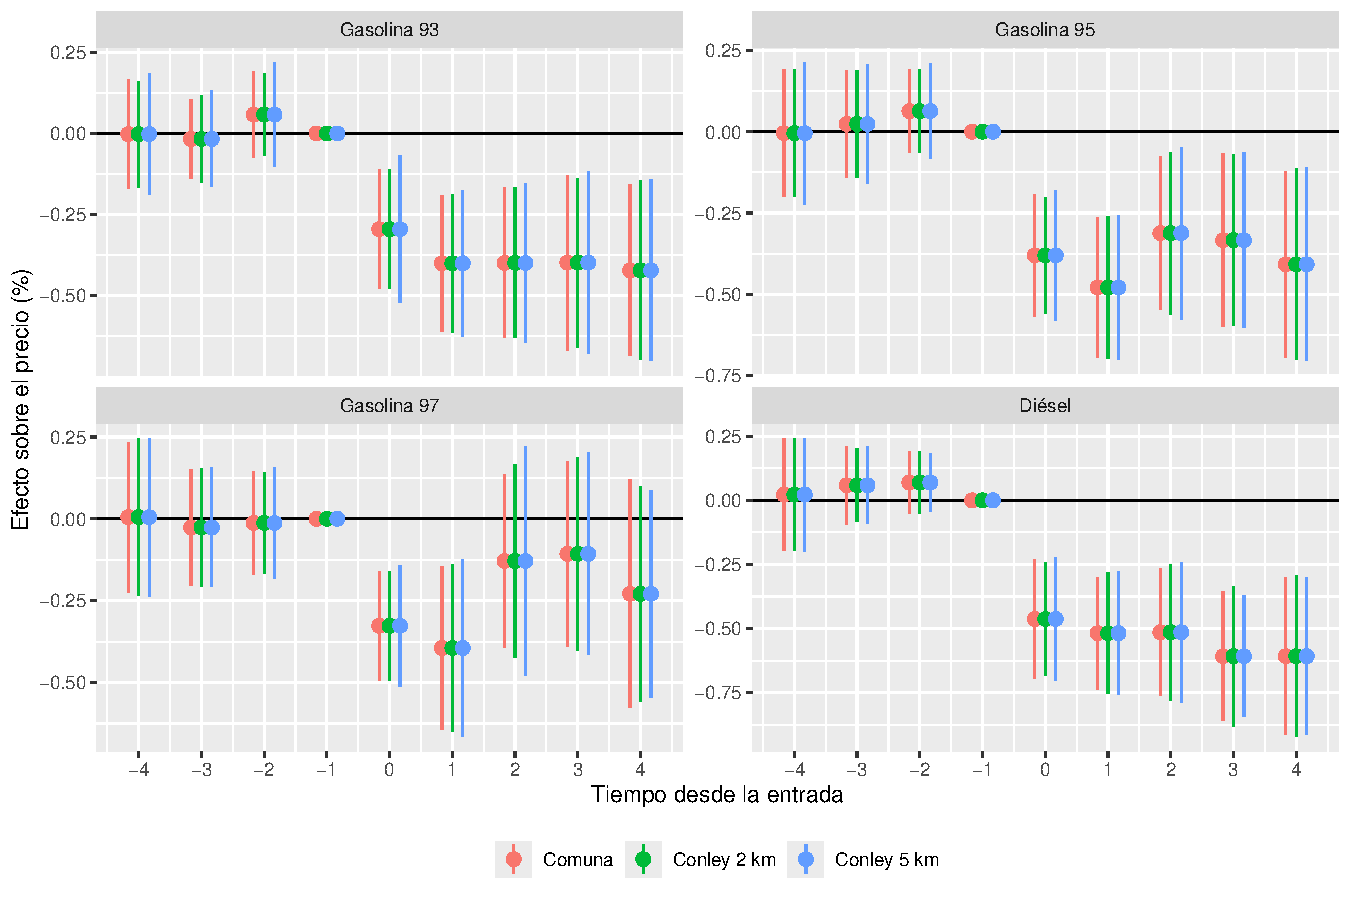
\includegraphics[width = \textwidth]{output/graficos/conley_2012_2026.pdf}
    \caption*{\footnotesize Fuente: Precios históricos de bencinaenlinea.cl. Log del precio $\times$ 100. Intervalos al 95\% con errores agrupados por comuna y de \textcite{CONLEY1991} con kernel uniforme y corte de 2 y 5 km. Bins de seis meses desde la entrada, extremos agrupados, referencia en $-1$. Control: estaciones sin entradas a menos de 5 km.}
\end{figure}

La Figura \ref{fig:fischer_semanal} repite el estudio de eventos principal con el diseño temporal de \textcite{FISCHER2025}: panel semanal, semana de la entrada, bins de 26 semanas y cohortes trimestrales en \textcite{SUNABRAHAM2021}. Los datos no permiten un panel diario, pues las estaciones reportan en promedio una vez por semana. Los coeficientes difieren en 0,04 puntos o menos de los mensuales. El efecto del primer semestre es algo menor en las gasolinas y el resto de los bins coincide.

\begin{figure}[htbp]
    \centering
    \caption{Estudio de eventos en panel mensual y semanal} \label{fig:fischer_semanal}
    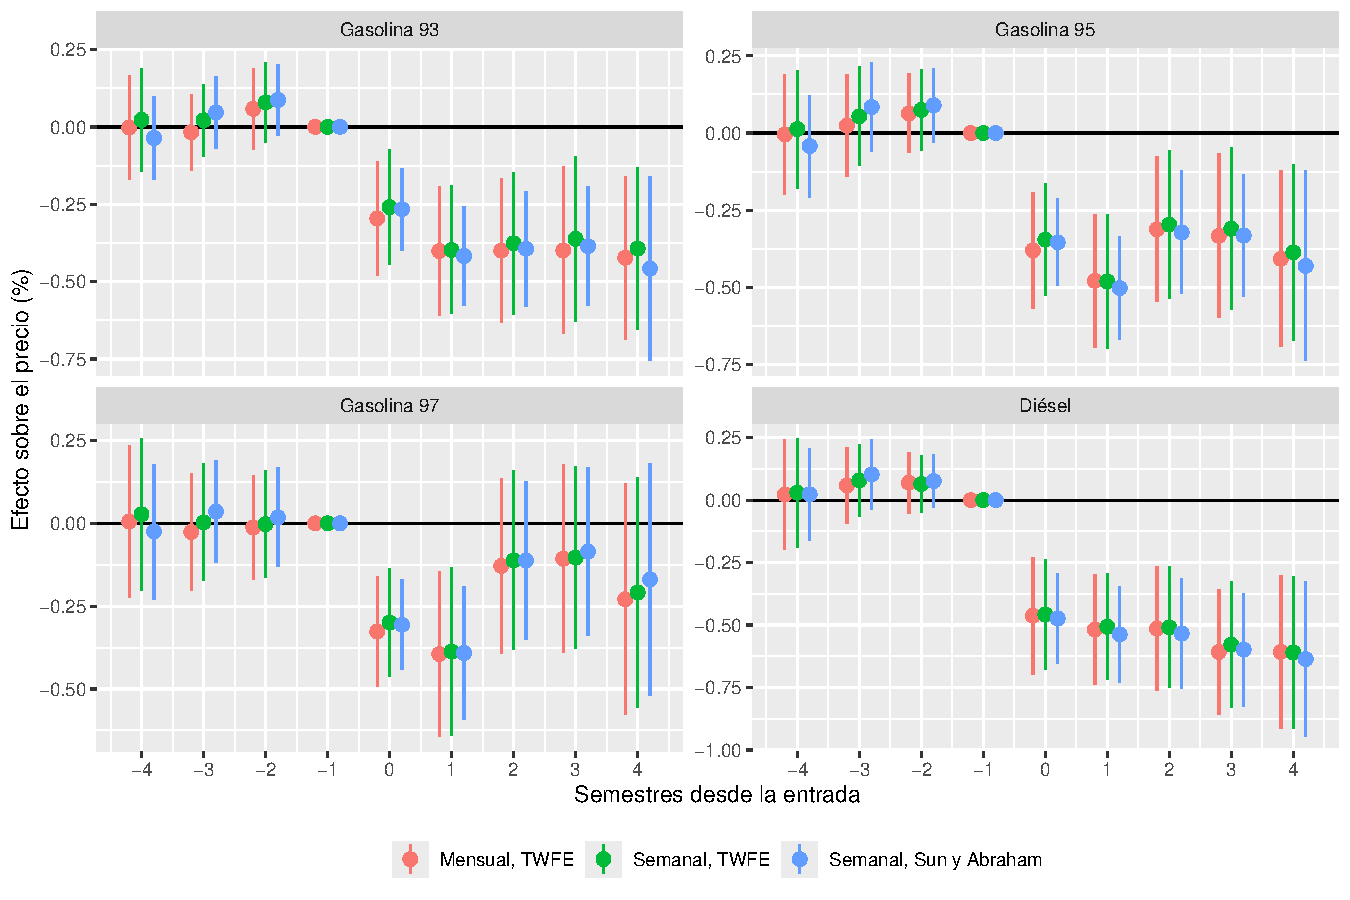
\includegraphics[width = \textwidth]{output/graficos/fischer_semanal.pdf}
    \caption*{\footnotesize Fuente: Precios históricos de bencinaenlinea.cl. Log del precio $\times$ 100. Mensual: especificación principal. Semanal: semana de la entrada, bins de 26 semanas, efecto fijo de semana y, en \textcite{SUNABRAHAM2021}, cohortes trimestrales, en gasolina 95 se excluye de este estimador una cohorte de dos estaciones cuyos coeficientes no están identificados. Extremos agrupados, referencia en $-1$. Efectos fijos de estación, región $\times$ año y marca $\times$ año. Intervalos al 95\% con errores estándar agrupados por comuna. Control: estaciones sin entradas a menos de 5 km.}
\end{figure}

\begin{figure}[htbp]
    \centering
    \caption{Estudio de eventos en estaciones de autopista y en el resto} \label{fig:het_autopista}
    
\includegraphics[width = \textwidth]{output/graficos/het_autopista.pdf}
    \caption*{\footnotesize Fuente: Precios históricos de bencinaenlinea.cl y red vial del MOP. Log del precio $\times$ 100. Tiempo desde la entrada interactuado con cada grupo en una sola regresión. Eje horizontal en semestres: bins de seis meses desde la entrada, extremos agrupados, referencia en $-1$. Mismas definiciones, muestra y efectos fijos que la Tabla \ref{tab:het_autopista}. Intervalos al 95\% con errores estándar agrupados por comuna.}
\end{figure}

\begin{figure}[htbp]
    \centering
    \caption{Efecto de la entrada sobre el número de estaciones del mercado local} \label{fig:persistencia}
    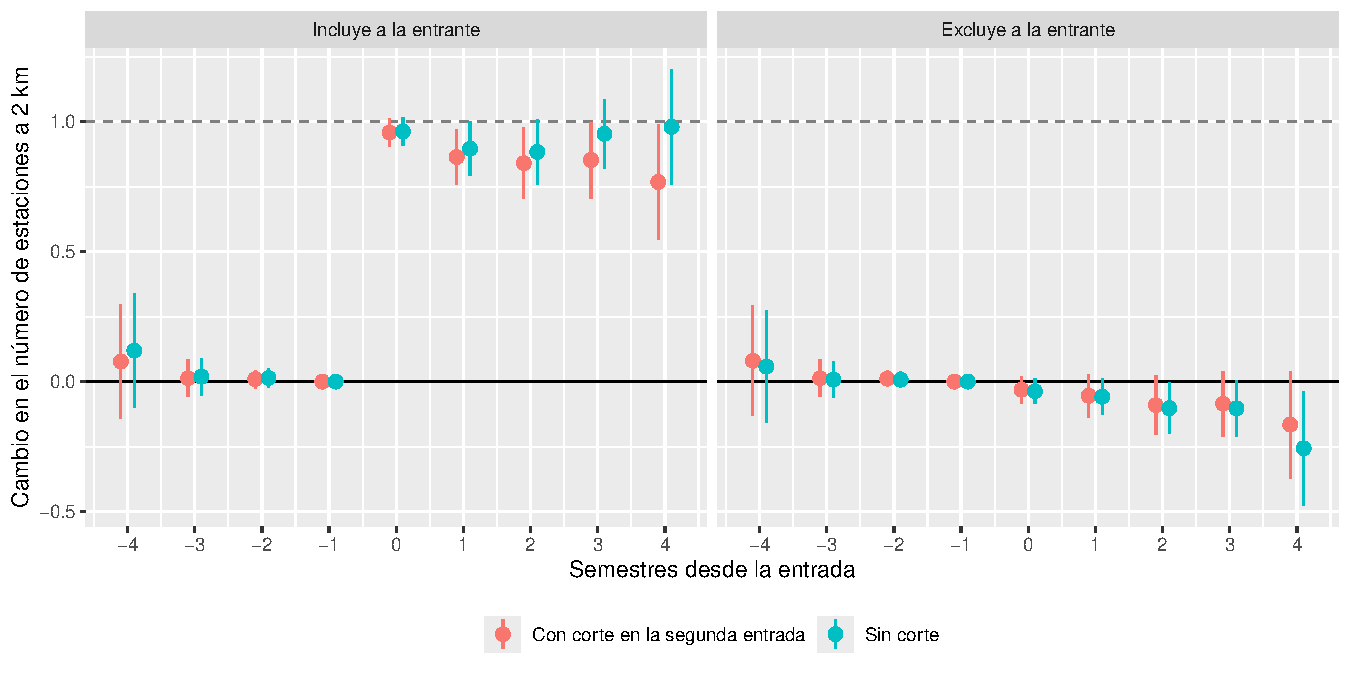
\includegraphics[width = \textwidth]{output/graficos/persistencia.pdf}
    \caption*{\footnotesize Fuente: Precios históricos de bencinaenlinea.cl. Estudio de eventos sobre el número de estaciones con registro a 2 km o menos de la incumbente, incluyendo y excluyendo a la entrante, con y sin el corte de la muestra en la segunda entrada. Eje horizontal en semestres: bins de seis meses desde la entrada, extremos agrupados, referencia en $-1$. La línea discontinua marca una estación adicional. Efectos fijos de estación, mes, región $\times$ año y marca $\times$ año. Intervalos al 95\% con errores estándar agrupados por comuna. Control: estaciones sin entradas a menos de 5 km.}
\end{figure}



\clearpage
\section{Tablas} \label{sec:anexo_tablas}

\begin{table}[h]
    \centering
    \caption{Composición de la muestra, ventana 2012 a 2026} \label{tab:composicion}
    \begin{tabular}{lr}
\toprule
 & N \\
\midrule
Estaciones observadas (2012--2026) & 2021 \\
\quad presentes en 2012 (incumbentes) & 1538 \\
\quad entrantes posteriores a 2012 & 483 \\
Entradas registradas & 483 \\
\quad cohortes focales (2014 en adelante) & 404 \\
Tratadas (entrada competidora a 2 km o menos) & 849 \\
Excluidas (entrada entre 2 y 3 km) & 261 \\
Control amplio (sin entradas a 3 km o menos) & 911 \\
\quad control estricto (sin entradas a 5 km o menos) & 662 \\
Muestra de estimación, gasolina 93 &  \\
\quad tratadas & 501 \\
\quad control amplio & 569 \\
\quad control estricto & 373 \\
\bottomrule
\end{tabular}

    \caption*{\footnotesize Fuente: Precios históricos de bencinaenlinea.cl.}
\end{table}

\begin{table}[h]
    \centering
    \caption{Estudio de eventos por grupo de control, gasolina 93} \label{tab:controles_p93}
    
\begingroup
\centering
\begin{tabular}{lcc}
   \toprule
                        & Control $>$3 km & Control $>$5 km \\   
                        & (1)             & (2)\\  
   \midrule 
   $\leq -4$            & 0.038           & -0.002\\   
                        & (0.088)         & (0.086)\\   
   $-3$                 & -0.010          & -0.017\\   
                        & (0.062)         & (0.062)\\   
   $-2$                 & 0.065           & 0.058\\   
                        & (0.066)         & (0.067)\\   
   $0$                  & -0.312$^{***}$  & -0.296$^{***}$\\   
                        & (0.091)         & (0.094)\\   
   $1$                  & -0.430$^{***}$  & -0.401$^{***}$\\   
                        & (0.104)         & (0.107)\\   
   $2$                  & -0.426$^{***}$  & -0.400$^{***}$\\   
                        & (0.109)         & (0.118)\\   
   $3$                  & -0.435$^{***}$  & -0.399$^{***}$\\   
                        & (0.130)         & (0.138)\\   
   $\geq 4$             & -0.479$^{***}$  & -0.423$^{***}$\\   
                        & (0.130)         & (0.135)\\   
   Tratadas             & 501             & 501\\  
   Controles            & 569             & 373\\  
    \\
   Observaciones        & 155,289         & 124,427\\  
    \\
   Estación             & Sí              & Sí\\  
   Mes                  & Sí              & Sí\\  
   Región $\times$ año  & Sí              & Sí\\  
   Marca $\times$ año   & Sí              & Sí\\  
   \bottomrule
\end{tabular}
\par\endgroup



    \notacontroles
\end{table}

\begin{table}[h]
    \centering
    \caption{Estudio de eventos por grupo de control, gasolina 97} \label{tab:controles_p97}
    
\begingroup
\centering
\begin{tabular}{lcc}
   \toprule
                        & Control $>$3 km & Control $>$5 km \\   
                        & (1)             & (2)\\  
   \midrule 
   $\leq -4$            & 0.059           & 0.005\\   
                        & (0.137)         & (0.117)\\   
   $-3$                 & -0.025          & -0.026\\   
                        & (0.088)         & (0.091)\\   
   $-2$                 & -0.025          & -0.013\\   
                        & (0.078)         & (0.080)\\   
   $0$                  & -0.320$^{***}$  & -0.327$^{***}$\\   
                        & (0.080)         & (0.085)\\   
   $1$                  & -0.401$^{***}$  & -0.395$^{***}$\\   
                        & (0.123)         & (0.128)\\   
   $2$                  & -0.155          & -0.129\\   
                        & (0.123)         & (0.134)\\   
   $3$                  & -0.176          & -0.107\\   
                        & (0.127)         & (0.144)\\   
   $\geq 4$             & -0.301$^{**}$   & -0.229\\   
                        & (0.148)         & (0.178)\\   
   Tratadas             & 471             & 471\\  
   Controles            & 500             & 313\\  
    \\
   Observaciones        & 135,630         & 107,247\\  
    \\
   Estación             & Sí              & Sí\\  
   Mes                  & Sí              & Sí\\  
   Región $\times$ año  & Sí              & Sí\\  
   Marca $\times$ año   & Sí              & Sí\\  
   \bottomrule
\end{tabular}
\par\endgroup



    \notacontroles
\end{table}

\begin{table}[h]
    \centering
    \caption{Estudio de eventos por grupo de control, diésel} \label{tab:controles_pdi}
    
\begingroup
\centering
\begin{tabular}{lcc}
   \toprule
                        & Control $>$3 km & Control $>$5 km \\   
                        & (1)             & (2)\\  
   \midrule 
   $\leq -4$            & 0.008           & 0.022\\   
                        & (0.106)         & (0.112)\\   
   $-3$                 & 0.045           & 0.059\\   
                        & (0.073)         & (0.078)\\   
   $-2$                 & 0.056           & 0.069\\   
                        & (0.061)         & (0.062)\\   
   $0$                  & -0.466$^{***}$  & -0.463$^{***}$\\   
                        & (0.121)         & (0.119)\\   
   $1$                  & -0.513$^{***}$  & -0.518$^{***}$\\   
                        & (0.113)         & (0.112)\\   
   $2$                  & -0.510$^{***}$  & -0.514$^{***}$\\   
                        & (0.126)         & (0.126)\\   
   $3$                  & -0.627$^{***}$  & -0.608$^{***}$\\   
                        & (0.130)         & (0.128)\\   
   $\geq 4$             & -0.623$^{***}$  & -0.608$^{***}$\\   
                        & (0.151)         & (0.157)\\   
   Tratadas             & 506             & 506\\  
   Controles            & 579             & 383\\  
    \\
   Observaciones        & 157,326         & 126,393\\  
    \\
   Estación             & Sí              & Sí\\  
   Mes                  & Sí              & Sí\\  
   Región $\times$ año  & Sí              & Sí\\  
   Marca $\times$ año   & Sí              & Sí\\  
   \bottomrule
\end{tabular}
\par\endgroup



    \notacontroles
\end{table}

\begin{table}[h]
    \centering
    \caption{Estudio de eventos por especificación de efectos fijos, gasolina 97} \label{tab:es_p97}
    
\begingroup
\centering
\begin{tabular}{lccccc}
   \toprule
                        & (1)             & (2)            & (3)            & (4)            & (5)\\  
   \midrule 
   $\leq -4$            & -5.164$^{***}$  & 0.260          & 0.298          & 0.083          & 0.005\\   
                        & (1.118)         & (0.234)        & (0.190)        & (0.121)        & (0.117)\\   
   $-3$                 & -1.625$^{*}$    & 0.218$^{*}$    & 0.189$^{*}$    & 0.006          & -0.026\\   
                        & (0.918)         & (0.115)        & (0.114)        & (0.091)        & (0.091)\\   
   $-2$                 & -0.512          & 0.159          & 0.136          & -0.001         & -0.013\\   
                        & (0.753)         & (0.099)        & (0.095)        & (0.080)        & (0.080)\\   
   $0$                  & -0.626          & -0.375$^{***}$ & -0.377$^{***}$ & -0.320$^{***}$ & -0.327$^{***}$\\   
                        & (0.803)         & (0.098)        & (0.093)        & (0.088)        & (0.085)\\   
   $1$                  & -0.742          & -0.530$^{***}$ & -0.508$^{***}$ & -0.381$^{***}$ & -0.395$^{***}$\\   
                        & (1.010)         & (0.178)        & (0.166)        & (0.130)        & (0.128)\\   
   $2$                  & -1.162          & -0.285         & -0.236         & -0.110         & -0.129\\   
                        & (1.408)         & (0.179)        & (0.159)        & (0.134)        & (0.134)\\   
   $3$                  & 0.004           & -0.220         & -0.154         & -0.093         & -0.107\\   
                        & (1.544)         & (0.176)        & (0.149)        & (0.148)        & (0.144)\\   
   $\geq 4$             & 21.161$^{***}$  & -0.356         & -0.356$^{**}$  & -0.211         & -0.229\\   
                        & (1.679)         & (0.309)        & (0.179)        & (0.182)        & (0.178)\\   
   Tratada              & -10.126$^{***}$ & -1.430$^{***}$ &                &                &   \\   
                        & (1.664)         & (0.381)        &                &                &   \\   
   Tratadas             & 472             & 472            & 471            & 471            & 471\\  
   Controles            & 318             & 318            & 313            & 313            & 313\\  
    \\
   Observaciones        & 107,258         & 107,258        & 107,252        & 107,252        & 107,247\\  
    \\
   Mes                  & No              & Sí             & Sí             & Sí             & Sí\\  
   Estación             & No              & No             & Sí             & Sí             & Sí\\  
   Región $\times$ año  & No              & No             & No             & Sí             & Sí\\  
   Marca $\times$ año   & No              & No             & No             & No             & Sí\\  
   \bottomrule
\end{tabular}
\par\endgroup



    \notaes
\end{table}

\begin{table}[h]
    \centering
    \caption{Estudio de eventos por especificación de efectos fijos, diésel} \label{tab:es_pdi}
    
\begingroup
\centering
\begin{tabular}{lccccc}
   \toprule
                        & (1)             & (2)            & (3)            & (4)            & (5)\\  
   \midrule 
   $\leq -4$            & -3.616$^{*}$    & 0.183          & 0.099          & 0.044          & 0.022\\   
                        & (1.942)         & (0.275)        & (0.139)        & (0.121)        & (0.112)\\   
   $-3$                 & -0.077          & 0.144          & 0.114          & 0.060          & 0.059\\   
                        & (1.735)         & (0.103)        & (0.092)        & (0.077)        & (0.078)\\   
   $-2$                 & 0.691           & 0.108$^{*}$    & 0.096          & 0.070          & 0.069\\   
                        & (1.056)         & (0.063)        & (0.060)        & (0.062)        & (0.062)\\   
   $0$                  & -2.898$^{**}$   & -0.501$^{***}$ & -0.520$^{***}$ & -0.478$^{***}$ & -0.463$^{***}$\\   
                        & (1.290)         & (0.141)        & (0.132)        & (0.121)        & (0.119)\\   
   $1$                  & -4.550$^{**}$   & -0.576$^{***}$ & -0.553$^{***}$ & -0.542$^{***}$ & -0.518$^{***}$\\   
                        & (2.013)         & (0.140)        & (0.117)        & (0.111)        & (0.112)\\   
   $2$                  & -6.113$^{**}$   & -0.617$^{***}$ & -0.508$^{***}$ & -0.538$^{***}$ & -0.514$^{***}$\\   
                        & (2.624)         & (0.180)        & (0.130)        & (0.128)        & (0.126)\\   
   $3$                  & -4.353$^{*}$    & -0.723$^{***}$ & -0.549$^{***}$ & -0.628$^{***}$ & -0.608$^{***}$\\   
                        & (2.589)         & (0.200)        & (0.150)        & (0.134)        & (0.128)\\   
   $\geq 4$             & 27.296$^{***}$  & -0.947$^{***}$ & -0.628$^{***}$ & -0.666$^{***}$ & -0.608$^{***}$\\   
                        & (2.353)         & (0.304)        & (0.178)        & (0.165)        & (0.157)\\   
   Tratada              & -12.444$^{***}$ & -1.558$^{***}$ &                &                &   \\   
                        & (2.239)         & (0.409)        &                &                &   \\   
   Tratadas             & 506             & 506            & 506            & 506            & 506\\  
   Controles            & 385             & 385            & 383            & 383            & 383\\  
    \\
   Observaciones        & 126,402         & 126,402        & 126,400        & 126,400        & 126,393\\  
    \\
   Mes                  & No              & Sí             & Sí             & Sí             & Sí\\  
   Estación             & No              & No             & Sí             & Sí             & Sí\\  
   Región $\times$ año  & No              & No             & No             & Sí             & Sí\\  
   Marca $\times$ año   & No              & No             & No             & No             & Sí\\  
   \bottomrule
\end{tabular}
\par\endgroup



    \notaes
\end{table}

\begin{table}[htbp]
    \centering
    \caption{Efecto de la entrada en estaciones de autopista y en el resto} \label{tab:het_autopista}
    
\begingroup
\centering
\begin{tabular}{lcccc}
   \toprule
                               & Gasolina 93    & Gasolina 95    & Gasolina 97          & Diésel \\   
                               & (1)            & (2)            & (3)                  & (4)\\  
   \midrule 
   Entrada                     & -0.526$^{***}$ & -0.544$^{***}$ & -0.371$^{***}$       & -0.660$^{***}$\\   
                               & (0.138)        & (0.149)        & (0.142)              & (0.162)\\   
   Entrada $\times$ autopista  & 0.756$^{***}$  & 0.832$^{***}$  & 0.933$^{***}$        & 0.644$^{*}$\\   
                               & (0.219)        & (0.229)        & (0.248)              & (0.383)\\   
   Efecto en autopista         & 0.230 (0.194)  & 0.287 (0.200)  & 0.562$^{**}$ (0.256) & -0.016 (0.360)\\  
   Tratadas resto              & 377            & 379            & 352                  & 381\\  
   Tratadas autopista          & 48             & 48             & 46                   & 48\\  
   Controles                   & 373            & 375            & 313                  & 383\\  
    \\
   Observaciones               & 113,466        & 112,886        & 96,934               & 115,229\\  
    \\
   Estación                    & Sí             & Sí             & Sí                   & Sí\\  
   Mes                         & Sí             & Sí             & Sí                   & Sí\\  
   Región $\times$ año         & Sí             & Sí             & Sí                   & Sí\\  
   Marca $\times$ año          & Sí             & Sí             & Sí                   & Sí\\  
   \bottomrule
\end{tabular}
\par\endgroup



    \caption*{\footnotesize Fuente: Precios históricos de bencinaenlinea.cl y red vial del MOP. Log del precio $\times$ 100. Autopista: incumbente a 100 m o menos del eje de la red vial primaria del MOP (clase 1). Entrada: efecto en el resto de las incumbentes, entrada $\times$ autopista: diferencia entre ambos grupos, efecto en autopista: suma de ambos, con su error estándar. Se excluyen las tratadas cuya entrante está a 100 m o menos de la red (77 de 506). Efectos fijos de estación, mes, región $\times$ año y marca $\times$ año. Errores estándar agrupados por comuna entre paréntesis. * p$<$0,10 ** p$<$0,05 *** p$<$0,01. Control: estaciones sin entradas a menos de 5 km.}
\end{table}

\begin{table}[htbp]
    \centering
    \caption{Efecto de la entrada sobre los precios del mercado local} \label{tab:mercado}
    \begin{tabular}{lcccc}
\toprule
 & Gasolina 93 & Gasolina 95 & Gasolina 97 & Diésel \\
\midrule
Percentil 90 & -0.291$^{***}$ & -0.242$^{*}$ & -0.028 & -0.457$^{***}$ \\
 & (0.111) & (0.124) & (0.164) & (0.124) \\
Mediana & -0.577$^{***}$ & -0.503$^{***}$ & 0.103 & -0.692$^{***}$ \\
 & (0.123) & (0.142) & (0.215) & (0.136) \\
Percentil 10 & -0.617$^{***}$ & -0.571$^{***}$ & -0.003 & -0.643$^{***}$ \\
 & (0.128) & (0.152) & (0.230) & (0.144) \\
\midrule
Tratadas & 445 & 449 & 397 & 451 \\
Controles & 191 & 188 & 161 & 191 \\
Observaciones & 88,888 & 88,726 & 75,067 & 89,529 \\
\bottomrule
\end{tabular}

    \caption*{\footnotesize Fuente: Precios históricos de bencinaenlinea.cl. ATT de Sun y Abraham en \% del cuantil del mercado (log del percentil 90, la mediana y el percentil 10 de los precios $\times$ 100). El mercado es el de la estación focal y estaciones con precio a 2 km o menos en el mes, incluida la entrante. Mercados con al menos una competidora en promedio antes de la entrada. Efectos fijos de estación, mes, región $\times$ año y marca $\times$ año. Controles son estaciones sin entradas a menos de 5 km. Errores estándar agrupados por comuna entre paréntesis. * p$<$0,10 ** p$<$0,05 *** p$<$0,01.}
\end{table}

La Tabla \ref{tab:validacion_margen} compara el margen de este trabajo, precio de venta menos el costo mayorista con MEPCO, con el margen contable que la \textcite{FNE2021informe} calcula para Copec, Petrobras y Shell en anillos de un kilómetro en torno a la ex estación Sesa de Av. Tobalaba 1895, entre agosto de 2018 y julio de 2019. El margen de este trabajo es parecido entre las tres marcas, entre 62 y 83 pesos por litro. El margen contable es menor en todas, y la diferencia es mayor en Shell y Petrobras (unos 40 pesos) que en Copec (unos 20 pesos). Como el precio de venta es casi igual entre marcas, la diferencia viene del costo: los costos de flete y almacenamiento son relevantes y no están incluidos en la referencia del MEPCO, y Copec tiene un costo de adquisición importantemente menor que el de sus competidoras, al menos en el mercado de este ejercicio.

\begin{table}[htbp]
    \centering
    \caption{Margen de este trabajo y margen contable de la FNE en torno a la ex estación Sesa} \label{tab:validacion_margen}
    \resizebox{\textwidth}{!}{\begin{tabular}{lcccccc}
\toprule
 & \multicolumn{2}{c}{Copec} & \multicolumn{2}{c}{Petrobras} & \multicolumn{2}{c}{Shell} \\
\cmidrule(lr){2-3} \cmidrule(lr){4-5} \cmidrule(lr){6-7}
Anillo & Este trabajo & FNE & Este trabajo & FNE & Este trabajo & FNE \\
\midrule
0--1 km & 9.4\% (62) & 5--10\% (40--50) & -- & -- & 9.4\% (62) & 0--5\% (20--30) \\
1--2 km & 9.9\% (66) & 5--10\% (50--60) & -- & -- & 9.5\% (63) & 0--5\% (20--30) \\
2--3 km & 10.4\% (69) & 5--10\% (40--50) & 9.6\% (63) & 0--5\% (20--30) & 10.6\% (71) & 0--5\% (20--30) \\
3--4 km & 10.7\% (71) & 5--10\% (40--50) & 11.0\% (74) & 0--5\% (20--30) & 10.2\% (68) & 0--5\% (20--30) \\
4--5 km & 12.2\% (83) & 5--10\% (50--60) & 10.2\% (68) & 5--10\% (30--40) & 10.5\% (71) & 0--5\% (20--30) \\
\bottomrule
\end{tabular}
}
    \caption*{\footnotesize Fuente: Precios históricos de bencinaenlinea.cl, costo mayorista con MEPCO y \textcite{FNE2021informe}, Tabla N.º 4. Margen porcentual sobre el precio de venta y, entre paréntesis, en pesos por litro, agosto de 2018 a julio de 2019. Este trabajo: precio menos costo mayorista con MEPCO, promedio simple de estación-mes de las gasolinas 93 y 97 y el diésel ponderadas por su participación nacional en volumen. FNE: ingresos menos costo de adquisición (precio de ENAP, impuesto específico, almacenamiento y transporte) sobre ingresos de las ventas minoristas de los cuatro combustibles, reportado en rangos. -- indica que no hay estaciones de la marca en el anillo.}
\end{table}

\begin{table}[htbp]
    \centering
    \caption{Sensibilidad del estudio de eventos principal, \textcite{RAMBACHAN2023}} \label{tab:honest_principal}
    \begin{tabular}{lcccc}
\toprule
 & Gasolina 93 & Gasolina 95 & Gasolina 97 & Diésel \\
\midrule
\multicolumn{5}{l}{\emph{Impacto (meses 0 a 5)}} \\
\quad Estimador & -0.296 & -0.380 & -0.327 & -0.463 \\
\quad IC 95\% & [-0.480, -0.111] & [-0.568, -0.192] & [-0.493, -0.160] & [-0.696, -0.229] \\
\quad $\bar{M}$ de quiebre & 1.00 & 1.75 & 1.25 & 2.25 \\
\multicolumn{5}{l}{\emph{Meses 6 a 11}} \\
\quad Estimador & -0.401 & -0.479 & -0.395 & -0.518 \\
\quad IC 95\% & [-0.611, -0.191] & [-0.694, -0.264] & [-0.645, -0.144] & [-0.737, -0.299] \\
\quad $\bar{M}$ de quiebre & 0.75 & 1.00 & 0.75 & 1.00 \\
\midrule
Tratadas & 501 & 503 & 471 & 506 \\
Controles & 373 & 375 & 313 & 383 \\
\bottomrule
\end{tabular}

    \caption*{\footnotesize Fuente: Precios históricos de bencinaenlinea.cl. Restricción de magnitudes relativas de \textcite{RAMBACHAN2023} sobre el estudio de eventos principal (log del precio $\times$ 100). Estimador e intervalo de confianza al 95\% convencional del bin indicado. $\bar{M}$ de quiebre: mayor $\bar{M}$ de la grilla de 0,25 a 3 con el que el intervalo robusto al 95\% excluye el cero. Control: estaciones sin entradas a menos de 5 km. Errores estándar agrupados por comuna.}
\end{table}

\begin{table}[htbp]
    \centering
    \caption{Sensibilidad del estudio de eventos sobre los precios del mercado local, \textcite{RAMBACHAN2023}} \label{tab:honest_mercado}
    \resizebox{\textwidth}{!}{\begin{tabular}{lcccccc}
\toprule
 & \multicolumn{3}{c}{Con entrante} & \multicolumn{3}{c}{Sin entrante} \\
\cmidrule(lr){2-4} \cmidrule(lr){5-7}
 & Percentil 90 & Mediana & Percentil 10 & Percentil 90 & Mediana & Percentil 10 \\
\midrule
\multicolumn{7}{l}{\emph{Gasolina 93}} \\
\quad Impacto (meses 0 a 5) & 0.25 & 0.50 & 1.00 & 0.25 & 0.25 & 0.50 \\
\quad Meses 6 a 11 & $<$0.25 & 0.75 & 0.75 & 0.25 & 0.75 & 0.50 \\
\multicolumn{7}{l}{\emph{Gasolina 95}} \\
\quad Impacto (meses 0 a 5) & 0.75 & 1.00 & 1.75 & 1.00 & 1.00 & 1.25 \\
\quad Meses 6 a 11 & 0.50 & 0.75 & 1.00 & 0.50 & 0.75 & 0.75 \\
\multicolumn{7}{l}{\emph{Gasolina 97}} \\
\quad Impacto (meses 0 a 5) & $<$0.25 & 0.25 & 1.50 & 0.25 & 0.75 & 1.00 \\
\quad Meses 6 a 11 & $<$0.25 & 0.25 & 0.75 & $<$0.25 & 0.25 & 0.50 \\
\multicolumn{7}{l}{\emph{Diésel}} \\
\quad Impacto (meses 0 a 5) & 0.50 & 1.25 & 1.25 & 0.50 & 1.25 & 0.75 \\
\quad Meses 6 a 11 & 0.25 & 1.00 & 0.50 & 0.25 & 0.75 & 0.50 \\
\bottomrule
\end{tabular}
}
    \caption*{\footnotesize Fuente: Precios históricos de bencinaenlinea.cl. $\bar{M}$ de quiebre de \textcite{RAMBACHAN2023}, restricción de magnitudes relativas, sobre el estudio de eventos TWFE del log del percentil 90, la mediana y el percentil 10 de los precios del mercado local. Con entrante incluye a la estación que abre, sin entrante la excluye. Mayor $\bar{M}$ de la grilla de 0,25 a 3 con el que el intervalo robusto al 95\% excluye el cero. Mercados de 2 km con al menos una competidora antes de la entrada. Control: estaciones sin entradas a menos de 5 km. Errores estándar agrupados por comuna.}
\end{table}

\begin{table}[htbp]
    \centering
    \caption{Placebo con fechas de entrada falsas asignadas al grupo de control} \label{tab:placebo_controles}
    \resizebox{\textwidth}{!}{\begin{tabular}{lcccc}
\toprule
 & Gasolina 93 & Gasolina 95 & Gasolina 97 & Diésel \\
\midrule
\multicolumn{5}{l}{\emph{Todo el grupo de control (386 estaciones)}} \\
\quad ATT placebo medio & 0.003 & 0.003 & -0.001 & 0.008 \\
\quad Desviación estándar de la distribución & 0.106 & 0.097 & 0.119 & 0.132 \\
\quad Error estándar agrupado medio & 0.103 & 0.092 & 0.111 & 0.133 \\
\quad Cociente error estándar / desviación & 0.98 & 0.95 & 0.93 & 1.01 \\
\quad Intervalo del 95\% de la distribución & [-0.215; 0.210] & [-0.190; 0.184] & [-0.247; 0.214] & [-0.237; 0.261] \\
\quad Tasa de rechazo al 5\% & 0.056 & 0.064 & 0.066 & 0.042 \\
\quad Valor $p$ por aleatorización del ATT real & 0.002 & 0.000 & 0.034 & 0.000 \\
\addlinespace
\multicolumn{5}{l}{\emph{Mitad más densa del grupo de control (194 estaciones)}} \\
\quad ATT placebo medio & 0.006 & 0.006 & 0.018 & 0.008 \\
\quad Desviación estándar de la distribución & 0.127 & 0.131 & 0.138 & 0.159 \\
\quad Error estándar agrupado medio & 0.114 & 0.119 & 0.124 & 0.146 \\
\quad Cociente error estándar / desviación & 0.90 & 0.91 & 0.90 & 0.92 \\
\quad Intervalo del 95\% de la distribución & [-0.254; 0.229] & [-0.259; 0.244] & [-0.244; 0.275] & [-0.313; 0.311] \\
\quad Tasa de rechazo al 5\% & 0.080 & 0.064 & 0.080 & 0.068 \\
\quad Valor $p$ por aleatorización del ATT real & 0.000 & 0.000 & 0.074 & 0.000 \\
\addlinespace
\midrule
ATT real & -0.397$^{***}$ & -0.404$^{***}$ & -0.243$^{**}$ & -0.587$^{***}$ \\
 & (0.111) & (0.118) & (0.119) & (0.128) \\
\bottomrule
\end{tabular}
}
    \caption*{\footnotesize Fuente: Precios históricos de bencinaenlinea.cl. 500 réplicas por grupo. En cada una se sortea como falsamente tratada la misma proporción de estaciones que en la muestra real, con cohortes y desfases a la segunda entrada sacados de sus distribuciones reales, y se estima el efecto estático de la especificación principal (log del precio $\times$ 100). Grupo de control: estaciones sin entradas a menos de 5 km, mitad más densa: estaciones con número de competidoras a 2 km o menos sobre la mediana del grupo. Error estándar agrupado medio: promedio del error agrupado por comuna entre réplicas, desviación estándar: dispersión de los 500 estimadores. Tasa de rechazo: proporción de réplicas con p $<$ 0,05. Valor $p$ por aleatorización: proporción de réplicas cuyo efecto iguala o supera en magnitud al efecto real. * p$<$0,10 ** p$<$0,05 *** p$<$0,01.}
\end{table}

\begin{table}[htbp]
    \centering
    \caption{Estudio de eventos con TWFE y Sun y Abraham, ventana 2014 a 2019} \label{tab:ventana_2014_2019}
    \resizebox{\textwidth}{!}{\begin{tabular}{lcccccccc}
\toprule
 & \multicolumn{2}{c}{Gasolina 93} & \multicolumn{2}{c}{Gasolina 95} & \multicolumn{2}{c}{Gasolina 97} & \multicolumn{2}{c}{Diésel} \\
\cmidrule(lr){2-3} \cmidrule(lr){4-5} \cmidrule(lr){6-7} \cmidrule(lr){8-9}
 & TWFE & SA & TWFE & SA & TWFE & SA & TWFE & SA \\
\midrule
$\leq -4$ & 0.127 & 0.143 & 0.255 & 0.320$^{***}$ & 0.309 & 0.521$^{***}$ & 0.149 & 0.206$^{*}$ \\
 & (0.143) & (0.091) & (0.186) & (0.106) & (0.213) & (0.154) & (0.152) & (0.119) \\
$-3$ & 0.090 & 0.112 & 0.187 & 0.222$^{**}$ & 0.235$^{*}$ & 0.325$^{***}$ & 0.111 & 0.119 \\
 & (0.129) & (0.109) & (0.151) & (0.113) & (0.136) & (0.101) & (0.160) & (0.140) \\
$-2$ & 0.134 & 0.156$^{*}$ & 0.139 & 0.161$^{**}$ & 0.161 & 0.213$^{***}$ & 0.117 & 0.131 \\
 & (0.112) & (0.086) & (0.108) & (0.078) & (0.118) & (0.078) & (0.103) & (0.087) \\
$0$ & -0.430$^{***}$ & -0.444$^{***}$ & -0.570$^{***}$ & -0.586$^{***}$ & -0.583$^{***}$ & -0.618$^{***}$ & -0.623$^{***}$ & -0.650$^{***}$ \\
 & (0.151) & (0.122) & (0.168) & (0.134) & (0.169) & (0.124) & (0.153) & (0.125) \\
$1$ & -0.616$^{***}$ & -0.617$^{***}$ & -0.746$^{***}$ & -0.749$^{***}$ & -0.713$^{***}$ & -0.734$^{***}$ & -0.811$^{***}$ & -0.851$^{***}$ \\
 & (0.164) & (0.123) & (0.197) & (0.142) & (0.207) & (0.133) & (0.188) & (0.154) \\
$2$ & -0.710$^{***}$ & -0.699$^{***}$ & -0.701$^{***}$ & -0.710$^{***}$ & -0.490$^{*}$ & -0.526$^{**}$ & -0.842$^{***}$ & -0.854$^{***}$ \\
 & (0.199) & (0.172) & (0.254) & (0.228) & (0.251) & (0.211) & (0.238) & (0.197) \\
$3$ & -0.618$^{***}$ & -0.619$^{***}$ & -0.702$^{***}$ & -0.735$^{***}$ & -0.477$^{***}$ & -0.554$^{***}$ & -0.830$^{***}$ & -0.826$^{***}$ \\
 & (0.170) & (0.102) & (0.185) & (0.137) & (0.173) & (0.154) & (0.185) & (0.131) \\
$\geq 4$ & -0.452$^{***}$ & -0.391$^{***}$ & -0.645$^{***}$ & -0.680$^{***}$ & -0.556$^{**}$ & -0.691$^{***}$ & -0.771$^{***}$ & -0.704$^{***}$ \\
 & (0.157) & (0.136) & (0.199) & (0.178) & (0.247) & (0.215) & (0.205) & (0.206) \\
\midrule
Tratadas & 453 & 453 & 456 & 456 & 418 & 418 & 459 & 459 \\
Controles & 672 & 672 & 682 & 682 & 557 & 557 & 697 & 697 \\
Observaciones & 75,343 & 75,343 & 75,710 & 75,710 & 63,411 & 63,411 & 77,210 & 77,210 \\
\bottomrule
\end{tabular}
}
    \caption*{\footnotesize Fuente: Precios históricos de bencinaenlinea.cl. Incumbentes presentes en 2014 y cohortes de entrada de 2015 a 2019. Log del precio $\times$ 100. SA: \textcite{SUNABRAHAM2021} con cohortes mensuales y las nunca tratadas como referencia. Bins de seis meses desde la entrada, extremos agrupados, referencia en $-1$. Efectos fijos de estación, mes, región $\times$ año y marca $\times$ año. Control: estaciones sin entradas a menos de 5 km. Errores estándar agrupados por comuna entre paréntesis. * p$<$0,10 ** p$<$0,05 *** p$<$0,01.}
\end{table}

\begin{table}[htbp]
    \centering
    \caption{Estudio de eventos con TWFE y Sun y Abraham, ventana 2021 a 2026} \label{tab:ventana_2021_2026}
    \resizebox{\textwidth}{!}{\begin{tabular}{lcccccccc}
\toprule
 & \multicolumn{2}{c}{Gasolina 93} & \multicolumn{2}{c}{Gasolina 95} & \multicolumn{2}{c}{Gasolina 97} & \multicolumn{2}{c}{Diésel} \\
\cmidrule(lr){2-3} \cmidrule(lr){4-5} \cmidrule(lr){6-7} \cmidrule(lr){8-9}
 & TWFE & SA & TWFE & SA & TWFE & SA & TWFE & SA \\
\midrule
$\leq -4$ & -0.004 & -0.018 & -0.157$^{*}$ & -0.171$^{***}$ & -0.275$^{**}$ & -0.269$^{***}$ & -0.025 & -0.024 \\
 & (0.121) & (0.070) & (0.091) & (0.065) & (0.138) & (0.079) & (0.124) & (0.095) \\
$-3$ & 0.005 & -0.011 & -0.003 & -0.014 & 0.015 & 0.022 & 0.087 & 0.080 \\
 & (0.071) & (0.044) & (0.064) & (0.045) & (0.106) & (0.051) & (0.088) & (0.070) \\
$-2$ & 0.005 & -0.003 & -0.004 & -0.007 & -0.004 & 0.003 & 0.003 & -0.003 \\
 & (0.061) & (0.031) & (0.072) & (0.033) & (0.109) & (0.036) & (0.075) & (0.038) \\
$0$ & -0.103 & -0.128$^{***}$ & -0.097 & -0.112$^{***}$ & -0.037 & -0.054 & -0.042 & -0.056 \\
 & (0.088) & (0.043) & (0.089) & (0.036) & (0.069) & (0.034) & (0.074) & (0.052) \\
$1$ & -0.196$^{*}$ & -0.230$^{***}$ & -0.202 & -0.239$^{***}$ & -0.062 & -0.109$^{**}$ & -0.194 & -0.215$^{**}$ \\
 & (0.101) & (0.060) & (0.129) & (0.074) & (0.075) & (0.049) & (0.147) & (0.084) \\
$2$ & -0.141 & -0.175$^{**}$ & -0.183 & -0.221$^{**}$ & 0.049 & -0.002 & -0.127 & -0.145 \\
 & (0.126) & (0.070) & (0.162) & (0.094) & (0.109) & (0.056) & (0.198) & (0.134) \\
$3$ & -0.039 & -0.090 & -0.049 & -0.112 & 0.340$^{**}$ & 0.285$^{**}$ & -0.067 & -0.105 \\
 & (0.110) & (0.075) & (0.138) & (0.096) & (0.159) & (0.139) & (0.226) & (0.156) \\
$\geq 4$ & -0.010 & 0.089 & -0.044 & 0.042 & 0.219$^{*}$ & 0.246$^{***}$ & -0.099 & -0.047 \\
 & (0.118) & (0.122) & (0.148) & (0.101) & (0.118) & (0.087) & (0.196) & (0.145) \\
\midrule
Tratadas & 195 & 195 & 196 & 196 & 180 & 180 & 199 & 199 \\
Controles & 1173 & 1173 & 1172 & 1172 & 1025 & 1025 & 1194 & 1194 \\
Observaciones & 75,570 & 75,570 & 75,364 & 75,364 & 67,073 & 67,073 & 76,987 & 76,987 \\
\bottomrule
\end{tabular}
}
    \caption*{\footnotesize Fuente: Precios históricos de bencinaenlinea.cl. Incumbentes presentes en 2021 y cohortes de entrada de 2022 a febrero de 2026. Log del precio $\times$ 100. SA: \textcite{SUNABRAHAM2021} con cohortes mensuales y las nunca tratadas como referencia. Bins de seis meses desde la entrada, extremos agrupados, referencia en $-1$. Efectos fijos de estación, mes, región $\times$ año y marca $\times$ año. Control: estaciones sin entradas a menos de 5 km. Errores estándar agrupados por comuna entre paréntesis. * p$<$0,10 ** p$<$0,05 *** p$<$0,01.}
\end{table}

